%!TEX root = ../main.tex
\chapter{ALGO_OPT}
\label{algo_opt}

\lhead{Chapitre ?? \emph{Chapter Title Here}}

\section{Non-Uniform time sampling algorithms}
\label{sec:time-sampling}

Two algorithms that automatically choose the time levels in order to
minimize the condition number are presented: first, the Almost
Periodic Fourier Transform (APFT) algorithm, initially proposed in the
 literature for electronics problems, is described, then a gradient-based
optimization algorithm over the condition number (OPT) is presented.


\subsection{The APFT algorithm}
\label{sec:apft-algorithm}

Based on the work of Kundert~\emph{et al.}~\cite{Kundert1988} in
electronics, the APFT algorithm has been implemented.  The aim of the
APFT algorithm is to maximize the orthogonality of the almost-periodic
DFT matrix in order to minimize its condition number.  It is based on
the Gram-Schmidt orthogonalization procedure.  First, the greatest
period $1/\min_k(f_k)$ is oversampled with $M$ equally-spaced time
levels, $M\gg2N+1$ being specified by the user and $N$ the number of
frequencies. Considering these time levels, a rectangular
almot-periodic IDFT matrix is built. Noting that every row of this
matrix is a vector, a set of $M$ vectors is obtained, numbered from 0
to $M-1$, and of length $2N+1$. The first vector $V_0$ (corresponding
to $t=0$) is arbitrarily chosen as the first time level and any
component in the direction of $V_0$ is removed from the following
vectors using the Gram-Schmidt formula:
\begin{equation}
   V_s = V_s - \frac{V_0^\top \cdot V_s}{V_0^\top \cdot V_0} V_0, \quad s=1,\cdots,M-1.
   \label{GramSchmidtAlgo}
\end{equation}
The remaining vectors are now orthogonal to $V_0$.  Since the vectors initially have the same Euclidean norm, the vector having the largest
norm is the most orthogonal to $V_0$.  It is assigned to $V_1$. The previous
operations are then performed on the $M-2$ remaining vectors using $V_1$
as $V_0$. This process is repeated until the required $2N+1$ vectors
are defined. As a time instant corresponds to a vector, $2N+1$ time levels are obtained, which enables the construction of the almost-periodic
DFT matrix. This algorithm is summarized in
Algo.~\ref{alg:algo_APFT}. % In order to further improve the results,
% the previous algorithm is embedded in an optimization algorithm that
% minimizes the condition number by looping on the over-sampling
% parameter $M$.

\begin{algorithm}[htb]
\caption{The Almost Periodic Fourier Transform Algorithm.}
\label{alg:algo_APFT}
\begin{algorithmic}
\STATE $\omega_{min} \leftarrow min \left( |\omega_k |,\quad 1 \leqslant k \leqslant N \right)$
\FOR{$m \leftarrow 0,\cdots,M-1$}
    \STATE $t_m \leftarrow \displaystyle\frac{2\pi}{\omega_{min}}\frac{m}{M}$
\ENDFOR
\FOR{$n \leftarrow 1,\cdots,2N$}
   \FOR{$m \leftarrow n+1,\cdots,M$}
  \STATE $ V_{m} \leftarrow V_{m} - \displaystyle\frac{V_{n}^\top \cdot V_{m}}{V_{n}^\top \cdot V_{n}} V_{n}$
   \ENDFOR
   \STATE \textbf{argmax()} returns the index of the largest member of a set
   \STATE $k=\textbf{argmax} \left( \| V_s^n \|,\quad n+1\leqslant s \leqslant M\right) $
   \STATE $\textbf{swap}(V_{n+1},V_{k})$
   \STATE $\textbf{swap}(t_{n+1},t_{k})$
\ENDFOR
\STATE $\mathbb{T}_{optimized} \leftarrow [t_0, \cdots, t_{2N}]$
\end{algorithmic}
\end{algorithm}

\subsection{Gradient-based optimization algorithm (OPT)}
A more direct approach is to seek directly a set of time levels
that minimize the condition number of the associated almost-periodic DFT matrix, 
instead of using orthogonality properties. 
This minimization problem can be solved numerically by 
an optimization algorithm. % A strategy based on an initial 
% sampling followed by a gradient-based method is now proposed.

The limited memory optimization method of
Broyden-Fletcher-Goldfarb-Shannon (L-BFGS-B, \cite{Byrd94alimited}) is
used to look for a minimum of the condition number of the
almost-periodic IDFT matrix $\kappa \left(A \left[\mathbb{T} \right]
\right)$ as function of the time levels vector $\mathbb{T}$.  This
quasi-Newton algorithm approximates the inverse Hessian matrix
$H(\kappa \left(A \left[\mathbb{T} \right] \right))^{-1}$ with the
BFGS formula in order to decrease the objective $\kappa \left(A
  \left[\mathbb{T} \right] \right)$ in the direction $-H(\kappa
\left(A \left[\mathbb{T} \right] \right))^{-1}\nabla \kappa \left(A
  \left[\mathbb{T} \right] \right)$.  This descent direction is
associated with the search for a zero of the gradient, which is a
necessary condition for an extremum, in a second order Taylor series.
Finally, a line search on $\alpha$ is performed to minimize $\kappa
\left(A \left[\mathbb{T} - \alpha H(\kappa \left(A \left[\mathbb{T}
      \right] \right))^{-1} \nabla \kappa \left(A \left[\mathbb{T}
      \right] \right) \right] \right)$.  In the present case, the
derivative $\nabla \kappa \left(A \left[\mathbb{T} \right] \right)$ of
the objective with respect to the time levels is approximated by
first-order finite differences.  An open-source implementation of this
reference broadly-used algorithm is
employed~\cite{Nocedal97lbfgsb}.

Gradient descent methods being local, the L-BFGS-B method converges to a local
minimum of the condition number.  This minimum is unsatisfying if the
starting point $\mathbb{T}$ is not well chosen, therefore a strategy
to find an appropriate one is required.  As shown in the following
comparison, APFT or uniform-sampling time levels do not always
guarantee acceptable condition numbers, and so cannot be used to
provide a starting point for L-BFGS-B. To this aim, the smallest
frequency is uniformly sampled:
\begin{equation}
    \Omega = [\frac{1}{M} \omega_{min}, \ldots, \frac{m+1}{M} \omega_{min}, \ldots, \omega_{min}],
    \label{eq:slitted_period}
\end{equation}
where $M$ denotes the desired number of initial guesses.
This gives a set of periods. Each of them are evenly sampled to obtain a
set of time levels. 
\begin{equation}
    \mathbb{T}_m = \left[ 0, \frac{2 \pi M}{ (2N + 1) (m+1) \omega_{min}}, \ldots, 
                             \frac{2N \pi M}{ (2N + 1) (m+1) \omega_{min}} \right]
    \label{eq:set_of_tlv}
\end{equation}

These time levels sets are then used as initial guesses for the
L-BFGS-B algorithm.

The almost-periodic IDFT matrix is built for
each of these time levels and the corresponding condition numbers are
computed.  A large number $M$, typically thousands, of fractions of the
greatest period gives a large set of potential time levels vectors.
This is acceptable given the very low cost of the computation of the
condition number on such small matrices of size $(2N + 1) \times
(2N+1)$.  From this set, the time levels vector associated with the
almost-periodic IDFT matrix having the smallest condition number is
taken as a starting point.  The optimization algorithm actually achieves
a local adjustment of the time levels.

In this way, the exploitation capability of the gradient-based
optimizer is well combined with the exploration capacity of the
sampling.  This finally gives solutions that are always close to the
ideal value of $1$, as shown in Tab.~\ref{tab:algo_sum}.  The OPT
method is summarized in Algo.~\ref{alg:algo_opt}.
\begin{algorithm}
\caption{The gradient-based optimization algorithm (OPT).}
\label{alg:algo_opt}
\begin{algorithmic}
\STATE $\omega_{min} \leftarrow min \left( |\omega_k |,\quad 1 \leqslant k \leqslant N \right)$
\FOR{$m \leftarrow 0,\cdots,M - 1$}
    \STATE $\omega_m \leftarrow \frac{m + 1}{M} \cdot \omega_{min}$
    \FOR{$i \leftarrow 0,\cdots,2N$}
        \STATE $t_i \leftarrow \displaystyle\frac{i \cdot 2 \pi}{\omega_m \cdot (2N + 1)}$
    \ENDFOR
    \STATE $\mathbb{T}_m \leftarrow [t_0, \cdots, t_i, \cdots, t_{2N}]$
    \STATE $C_m \leftarrow \kappa \left(A \left[\mathbb{T}_m \right] \right)$
\ENDFOR
\STATE \textbf{argmin()} returns the index of the smallest member of a set
\STATE $k \leftarrow \textbf{argmin}\left(C_m,\quad 0\leqslant m \leqslant M-1\right)$
\STATE $\textbf{min\_l-bfgs-b}\left(\kappa \left(A\left[\mathbb{T}\right]\right), \mathbb{T}_{ini}\right)$ returns the optimal 
time levels vector $\mathbb{T}$ with the condition number $\kappa\left(A\left[\mathbb{T}\right]\right)$ as objective function 
using the L-BFGS-B algorithm and  $\mathbb{T}_{ini}$ as starting point.
\STATE $\mathbb{T}_{optimized} \leftarrow \textbf{min\_l-bfgs-b}\left(\kappa\left(A\left[\mathbb{T}\right]\right), \mathbb{T}_{ini}=\mathbb{T}_k\right)$
\end{algorithmic}
\end{algorithm}

\subsection{Assessment of the algorithms}

Let us consider the case of two frequencies, $f_1$ and $f$. 
Without loss of generality it can be assumed that $f \leq f_1$.
The non-dimensional frequency $\delta_f^*$ is defined as:
% To assess the presented algorithms, a model problem for two frequencies $f_1$ and $f_2$ is considered.
% As the absolute value of the frequencies is not relevant, the space of parameters is mapped by a non-dimensional
% frequency~$\delta_f^*$, defined as:
\begin{equation}
    \delta_f^* \colon\begin{cases}
        [0: f_1] & \longmapsto[0: 2]\\
        f & \longmapsto 2 \cdot \displaystyle \frac{f_1 - f}{f_1 + f}
    \end{cases}
    \label{eq:delta_f}
\end{equation}
By taking $f_1$ constant, and having $\delta_f^*$ sampled between $0$
and $2$, the whole range of $f \leq f_1$ is explored. Moreover, as
$\delta_f^*$ is anti-symmetric ($\delta_f^*(-f) = - \delta_f^*(f)$), and as the almost-periodic IDFT matrix is symmetric $A[-f] = A[f]$, the following relation is obtained for the condition number:
\begin{equation}
  \kappa \left(A \left[\delta_f^*\left(-f\right)\right]\right) =
  \kappa \left(A \left[-\delta_f^*\left(f\right)\right]\right) 
  = \kappa \left(A \left[\delta_f^*\left(f\right)\right]\right),
  \label{eq:permutation}
\end{equation}
meaning that the case $f\geq f_1$ can be deduced in a straightforward
way.

For each value of $\delta_f^*$, the condition number of the
almost-periodic IDFT matrix $\kappa ( A )$ is computed, highlighting
the ability of the different algorithms to choose the time levels that
minimize the condition number, for any input frequencies. This
assessment is only valid for two frequencies, but the tendency is similar
when increasing the number of frequencies. Two frequencies are
involved thus five time levels are required. The results of three
algorithms are depicted Fig.~\ref{fig:bench_algo}: (i)~APFT: the
Almost Periodic Fourier Transform algorithm, (ii)~OPT: the
gradient-based optimization algorithm and (iii)~EQUI: evenly spaced
time levels oversampling the largest period as done in
Gopinath~\emph{et al.}~\cite{gopinath2007three} using $2N+1$ time
levels and in Ekici and Hall~\cite{Ekici2007, Ekici2008} using $3N+1$
time levels.
\begin{figure}[htb]
  \centering 
    \subfigure[Evenly-spaced time levels
    algorithms]{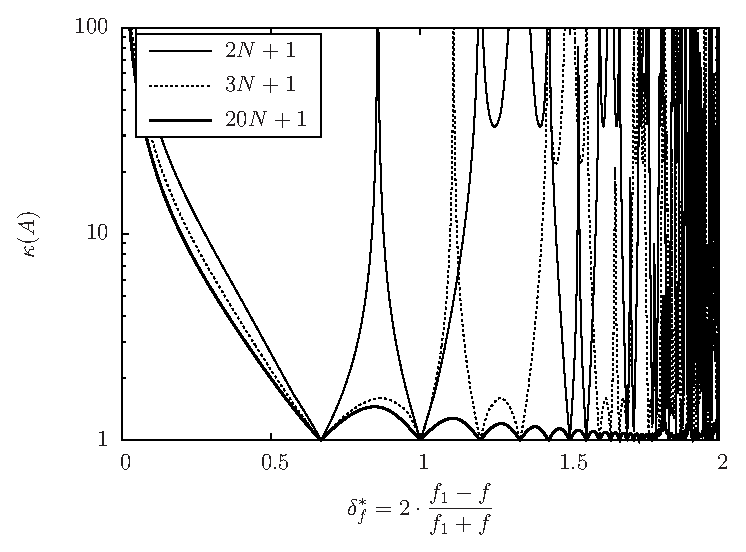
\includegraphics[width=.45\textwidth]{NONEQUI_BENCH_EQUI.eps}}
    \quad\subfigure[Proposed
    algorithms]{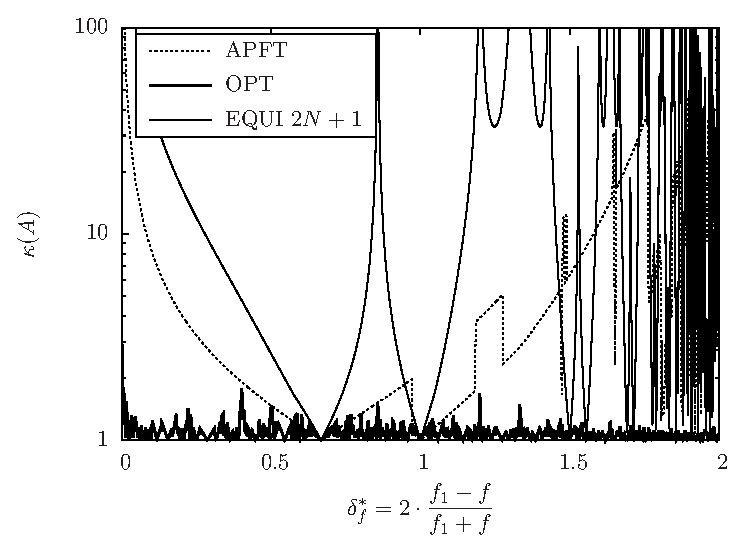
\includegraphics[width=.45\textwidth]{NONEQUI_BENCH_ALGO.eps}}
  \caption{Comparison of the presented algorithms.}
  \label{fig:bench_algo}
\end{figure}

The EQUI algorithms give fair results ($\kappa(A) \leq 2$) only at
discrete points, corresponding to the particular cases where $f$ is a
multiple of $f_1$, which are thus similar to the single-frequency
case. Oversampling improves the results. In fact, the mean condition number obtained
with $20N + 1$ time levels indicates that the higher the number of time levels
the better the condition number. However the almost-periodic DFT
matrix becomes rectangular and the memory cost of such a computation
increases drastically, preventing the use of such an approach on industrial cases. The APFT
algorithm improves the results, as it gives results with $\kappa ( A
)$ close to unity for $0.3 \leq \delta_f^* \leq 1.2$. However, when
$\delta_f^*$ tends to the boundaries (0 and~2), the condition
number seems to go to infinity. This corresponds to special values
of~$f$:
\begin{equation}
  \begin{split}
    \delta_f^* = 0 & \iff f = f_1, \\
    \delta_f^* = 2 & \iff f = 0. \\
  \end{split}
  \label{eq:singularities}
\end{equation}
This means that the APFT algorithm fails to work when the frequencies
are too close to one another, and when they are significantly
different.  This limits the method for a range of frequencies where
the HB method could give a salient gain in CPU time. %
%Actually, if the frequencies 
%have more than one order of magnitude difference, a classical time marching scheme
%would have to discretize the smallest period and run the simulation long enough to have
%the longest period converged, increasing drastically
%the computational time. On the opposite, the presented HB
%approach does not rely on an over-sampling. Hence its gain in CPU time.
Finally, the OPT algorithm gives a condition number close to unity for
any value of $\delta_f^*$. The OPT algorithm thus ensures that the
convergence of the HB method is not sensitive to the specified set of
frequencies. Table~\ref{tab:algo_sum} summarizes the results obtained
with each algorithm.
\begin{table}[htb]
  \centering
  \begin{tabular}{|r|*{5}{c|}}
    \hline
    & \multicolumn{3}{c|}{EQUI} & APFT & OPT\\
    \hline
    \# instants & $2N+1$ & $3N+1$ & $20N+1$ & $2N+1$ & $2N+1$ \\
    \hline
    \hline
    $\min \left( \kappa \left[A\right]\right) $ & $1.002$ & $1.0$ & $1.0$ & $1.001$ & $1.000$ \\
    \hline
    $\max \left( \kappa \left[A\right]\right) $ & $3.024\cdot 10^{14}$ & $1.871\cdot 10^{11}$ & $2732.6$ & $823.8$ & $2.905$ \\
    \hline
    $\textrm{mean} \left( \kappa \left[A\right]\right) $ & $3.081\cdot 10^{11}$ & $1.871\cdot 10^{8}$ & $10.92$ & $7.742$ & $1.097$ \\
    \hline
  \end{tabular}
\caption{Global results for the presented algorithms.}
\label{tab:algo_sum}
\end{table} 

Thus the proposed non-uniform time sampling combined with the OPT
algorithm allows to tackle problems with large frequency
separation. In such cases, the gain of the HB approach compared
to classical time-marching methods is expected to be significant: with
a time-marching scheme, the time-step has to be small enough to
discretize the shortest period, while the number of time steps of the
simulation has to be long enough to reach the (almost-)periodic state
(\emph{i.e.}  the simulation time is equal to several
times the longest period). Conversely, the cost of the HB method only
depends on the number of frequencies to capture, regardless of their
relative values.
%the longest period converged, increasing drastically
%the computational time.

\subsection{Distribution of the time levels}

For harmonically-related frequencies, the optimal time levels
correspond to a uniform set sampling the fundamental frequency period
as it gives the theoretical lower bound $\kappa (A) = 1$. Since the
frequencies are harmonically related, the distribution of the time
levels on the other frequencies is also uniform. Considering the
frequency vector $F = \left[f_1, \cdots,f_k= kf_1,\ldots,Nf_1 \right]$
and the time levels vector
$\mathbb{T}$:% evenly spaced on the first harmonic period:
\begin{equation}
  \mathbb{T} = \left[0, \frac{1}{f_1\cdot(2N+1)}, \cdots,  \frac{2N}{f_1\cdot(2N+1)} \right],
  \label{eq:evenly_spaced_timelevels}
\end{equation}
then the product of the $i^{th}$ term of $\mathbb{T}$ to its
associated frequency is
\begin{equation}
  f_1 \cdot \frac{i}{f_1\cdot(2N+1)} = k f_1 \cdot \frac{i}{k f_1 \cdot (2N+1)} = f_k \cdot \frac{i}{f_k\cdot(2N+1)}.
  \label{eq:evenly_spaced_timelevels_2}
\end{equation}
Eq.~\eqref{eq:evenly_spaced_timelevels_2} means that evenly-spaced
time levels for the fundamental frequency are still seen as evenly
spaced by the $k^{th}$ harmonic. This is an explanation why the
condition number of the almost-periodic IDFT matrix $A^{-1}$ will be
unity as each frequency is sampled by evenly spaced time
levels~\cite{Brambilla:1999fk}.

Now, considering non-harmonically related frequencies, there is
mathematically no reason for evenly-spaced time levels over the
smallest frequency to be seen as evenly spaced by the other frequencies
in general. Therefore, the use of non-evenly spaced time levels,
  and algorithms to automatically choose them, becomes necessary.

Figure~\ref{fig:distribution_tlv} shows the distribution of the time
levels, relative to each frequency period, obtained by the presented
algorithms for the frequencies $f_1 = 3$~Hz and $f_2 = 17$~Hz (\emph{i.e.}
$\delta_f^*=1.4$).  To do so, the chosen time levels are redistributed
on the considered frequency period by applying a modulo to it:
\begin{equation}
  \label{eq:1}
  \mathbb{T}^{[f_k]}_j =  \mathbb{T}_j \text{ modulo } 1/f_k
\end{equation}
Then, they are divided by the latter, so that the results are
dimensionless.  In light gray line is depicted the $y=x$ function
representing the evenly-spaced solution on the considered period.
Keeping in mind that if each frequency sees evenly-spaced time levels,
then the condition number is the smallest, the optimal solution would
be to have relative time levels on $y=x$ for each period.  Running the
EQUI, APFT and OPT algorithms leads to a condition number of $33.1$,
$3.8$ and $1.1$, respectively.  The EQUI algorithm is perfect for the
period $1/f_1$ but is really far from the evenly spaced time levels
for period $1/f_2$. The APFT algorithm is far from the evenly spaced
solution for both the periods considered, but closer than EQUI regarding
period $1/f_2$. Finally, the OPT algorithm is the only one to be close
to the evenly spaced solution for each considered period, allowing 
the proposed HB method to be used for any set of frequencies.
\begin{figure}[htb]
  \centering \subfigure[Relative to period
  $1/f_1$]{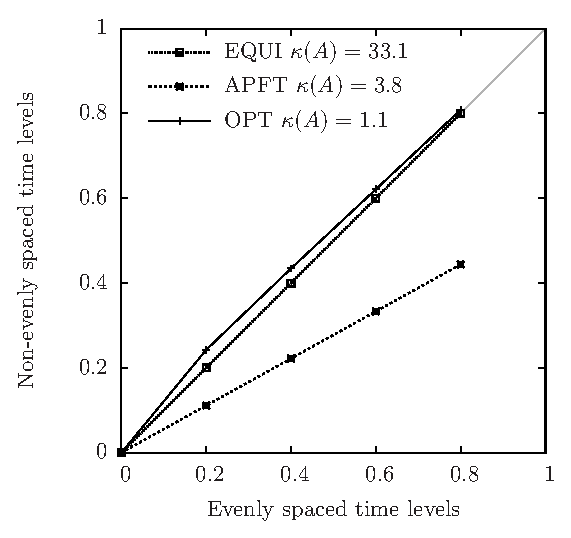
\includegraphics[width=.45\textwidth]{NONEQUI_TIMELEVELS_POSITION_F1.eps}}
  \quad\subfigure[Relative to period
  $1/f_2$]{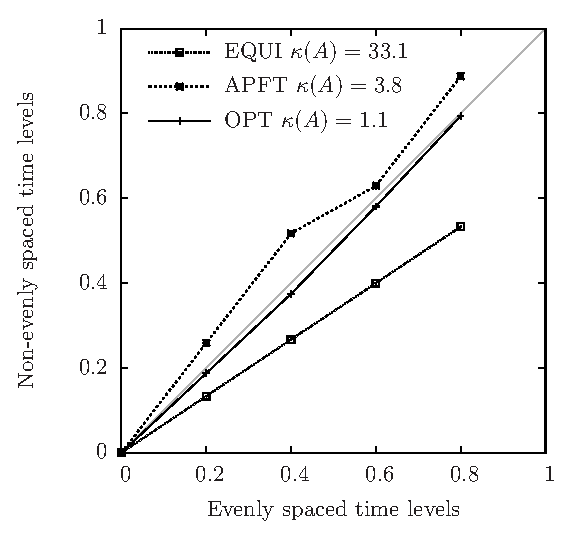
\includegraphics[width=.45\textwidth]{NONEQUI_TIMELEVELS_POSITION_F2.eps}}
  \caption{Distribution of the time levels on each frequency periods.}
  \label{fig:distribution_tlv}
\end{figure}

The source code of the proposed algorithms and the scripts to generate
Figures~\ref{fig:bench_algo} and~\ref{fig:distribution_tlv} are available
over the internet\,\footnote{\url{http://cerfacs.fr/~gomar/PyLeap.html}}.


%The behavior of these algorithms are now experimented on HB computation
%of a channel flow with fluctuating pressure outlet.
The impact of the time sampling on HB computations is now investigated
for the simple case of a channel flow with fluctuating pressure
outlet.